\documentclass{article}
\usepackage{polski}
\usepackage[utf8]{inputenc}
\usepackage{natbib}
\usepackage{graphicx}
\usepackage{xcolor}
\usepackage{mathtools}
\usepackage{amssymb}
\usepackage[makeroom]{cancel}
\usepackage{hyperref}
\newcommand{\norm}[1]{\left\lVert#1\right\rVert}


\title{Sprawozdanie 3}
\author{Jan Bronicki 249011}
\date{}


\begin{document}

\maketitle

\section{Zadanie}

Zadanie: Opisać schemat, policzyć, wyznaczyć parametry i przesymulować układ 4..20mA dla
wybranych 3 wartości Rpom i dla nich określić : max wartość Robc dla I=4:20mA, wykonać wykres
Uster(Uce), Uce(Robc), Robc(Pdiss) dla wybranych Robc oraz Iz (x3).

\section{Moduł 4..20mA}

\subsection{NPN}

\begin{itemize}
    \item Schemat
        \begin{figure}[h!]
            \centering
            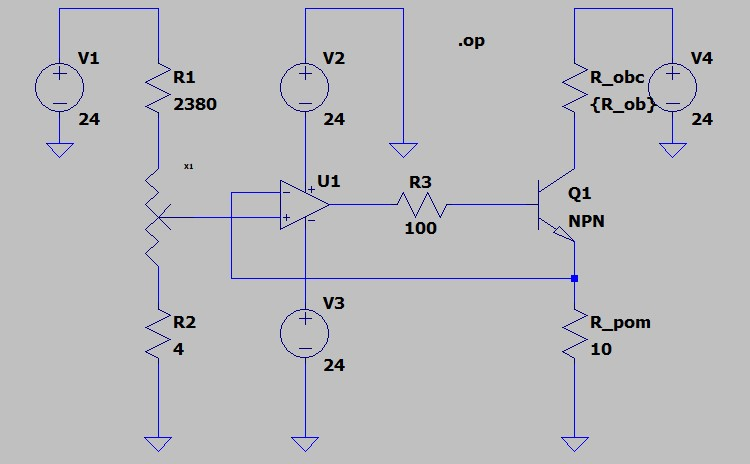
\includegraphics[scale=0.4]{main_schemat.jpg}
        \end{figure}
    \item Wyznaczenie parametrów
\end{itemize}

\newpage


\subsubsection{$R_{pom} = 10 \Omega$}


Wybrana wartość, dla $R_{3} = 100 \Omega$

Zakres napięcia do sterowania:

$$
    I_{min} = 4mA \rightarrow U_{4mA} = 4mA \cdot 10 \Omega = 0.04V
$$
$$
    I_{max} = 20mA \rightarrow U_{20mA} = 20mA \cdot 10 \Omega = 0.2V
$$

Maksymalne wartości $R_{obc}$, czyli $R_{max}$:

$$
    R_{max} = \frac{24V-U_{CE_{min}}-R_{pom}\cdot I_{max}}{I_{max}}
$$

Aby wartość $U_{CE} \geq 0.1V$, gdzie $I_{max}=20mA$:

$$
    R_{max}=\frac{24V-0.1V-10\Omega \cdot 20mA}{20mA}=1185\Omega
$$

Przyjęta wartość, dla $R_{obc} = 1000 \Omega, \ \ I_{sterowania} = 4mA$:

$$
    R_{1} = \frac{24V - U_{20mA}}{I_{sterowania}}=\frac{24V - 0.2V}{4mA} = 5950 \Omega
$$

$$
    R_{pot} = \frac{U_{20mA} - U_{4mA}}{I_{sterowania}} = 
    \frac{0.20V-0.04V}{4mA} 40\Omega
$$


$$
    R_{2} = \frac{U_{4mA}}{I_{sterowania}} = \frac{0.04V}{10mA} = 10 \Omega
$$

Schemat:\\
Wykresy:

\begin{itemize}
    \item $U_{ster}(U_{CE})$
    \item $U_{CE}(R_{obc}), gdzie Val = 50, \ \ R_{max} = 1981 \Omega$
\end{itemize}






\newpage
\subsubsection{$R_{pom} = 100 \Omega$}


Przyjęte $R_{obc} = 1000 \Omega$:


Wartość, dla $R_{3} = 100 \Omega$

Napięcie do sterowania:

$$
I_{min} = 4mA \rightarrow U_{4mA} = 4mA \cdot 100 \Omega = 0.4V
$$
$$
I_{max} = 20mA \rightarrow U_{20mA} = 20mA \cdot 100 \Omega = 2V
$$

Sterowanie: $I_{sterowania} = 4mA$:

$$
    R_{1} = \frac{24V - U_{20mA}}{I_{sterowania}}=\frac{24V - 2V}{4mA} = 5500 \Omega
$$

$$
    R_{pot} = \frac{U_{20mA} - U_{4mA}}{I_{sterowania}} = 
    \frac{2V-0.4V}{4mA} = 400 \Omega
$$


$$
    R_{2} = \frac{U_{4mA}}{I_{sterowania}} = \frac{0.4V}{4mA} = 100 \Omega
$$

Schemat:

Wykresy:

\begin{itemize}
    \item $U_{ster}(U_{CE})$
    \item $U_{CE}(R_{obc}), gdzie Val = 50, \ \ R_{max} = 1891 \Omega$
    \item $R_{obc}(P_{diss}), gdzie Val = 50, \ \ R_{max} =1891 \Omega$
\end{itemize}


\subsubsection{$R_{pom} = 200 \Omega$}

Wartość, dla $R_{3} = 100 \Omega$

Napięcie do sterowania:

$$
    I_{min} = 4mA \rightarrow U_{4mA} = 4mA \cdot 200 \Omega = 0.8V
$$
$$
    I_{max} = 20mA \rightarrow U_{20mA} = 20mA \cdot 200 \Omega = 4V
$$



$R_{obc} = 800 \Omega$

Pozostałe wartości rezystorów, dla $I_{sterowania} = 4mA$:


$$
    R_{1} = \frac{24V - U_{20mA}}{I_{sterowania}}=\frac{24V - 4V}{4mA} = 5000 \Omega
$$

$$
    R_{pot} = \frac{U_{20mA} - U_{4mA}}{I_{sterowania}} = 
    \frac{4V-0.8V}{4mA} = 800 \Omega
$$


$$
    R_{2} = \frac{U_{4mA}}{I_{sterowania}} = \frac{0.8V}{10mA} = 200 \Omega
$$

Schemat:

Wykresy:


\begin{itemize}
    \item $U_{ster}(U_{CE})$
    \item $U_{CE}(R_{obc}), gdzie Val = 50, \ \ R_{max} = 1791 \Omega$
    \item $R_{obc}(P_{diss}), gdzie Val = 50, \ \ R_{max} =1791 \Omega$
\end{itemize}




\subsection{PNP}

\begin{itemize}
    \item Schemat
    \item Wyznaczenie parametrów
\end{itemize}

\section{Wnioski}

\end{document}